\section{System Overview}

The system consists of four main parts:
\begin{enumerate}
    \item The communications system between the FPGA and the MCU
    \item The Framebuffer
    \item The Display Driver
    \item The Render Pipeline
\end{enumerate}

The following is a diagram of the entire system, it's parts, and the 
dataflow between modules.

\begin{figure}[H]
    \centering
    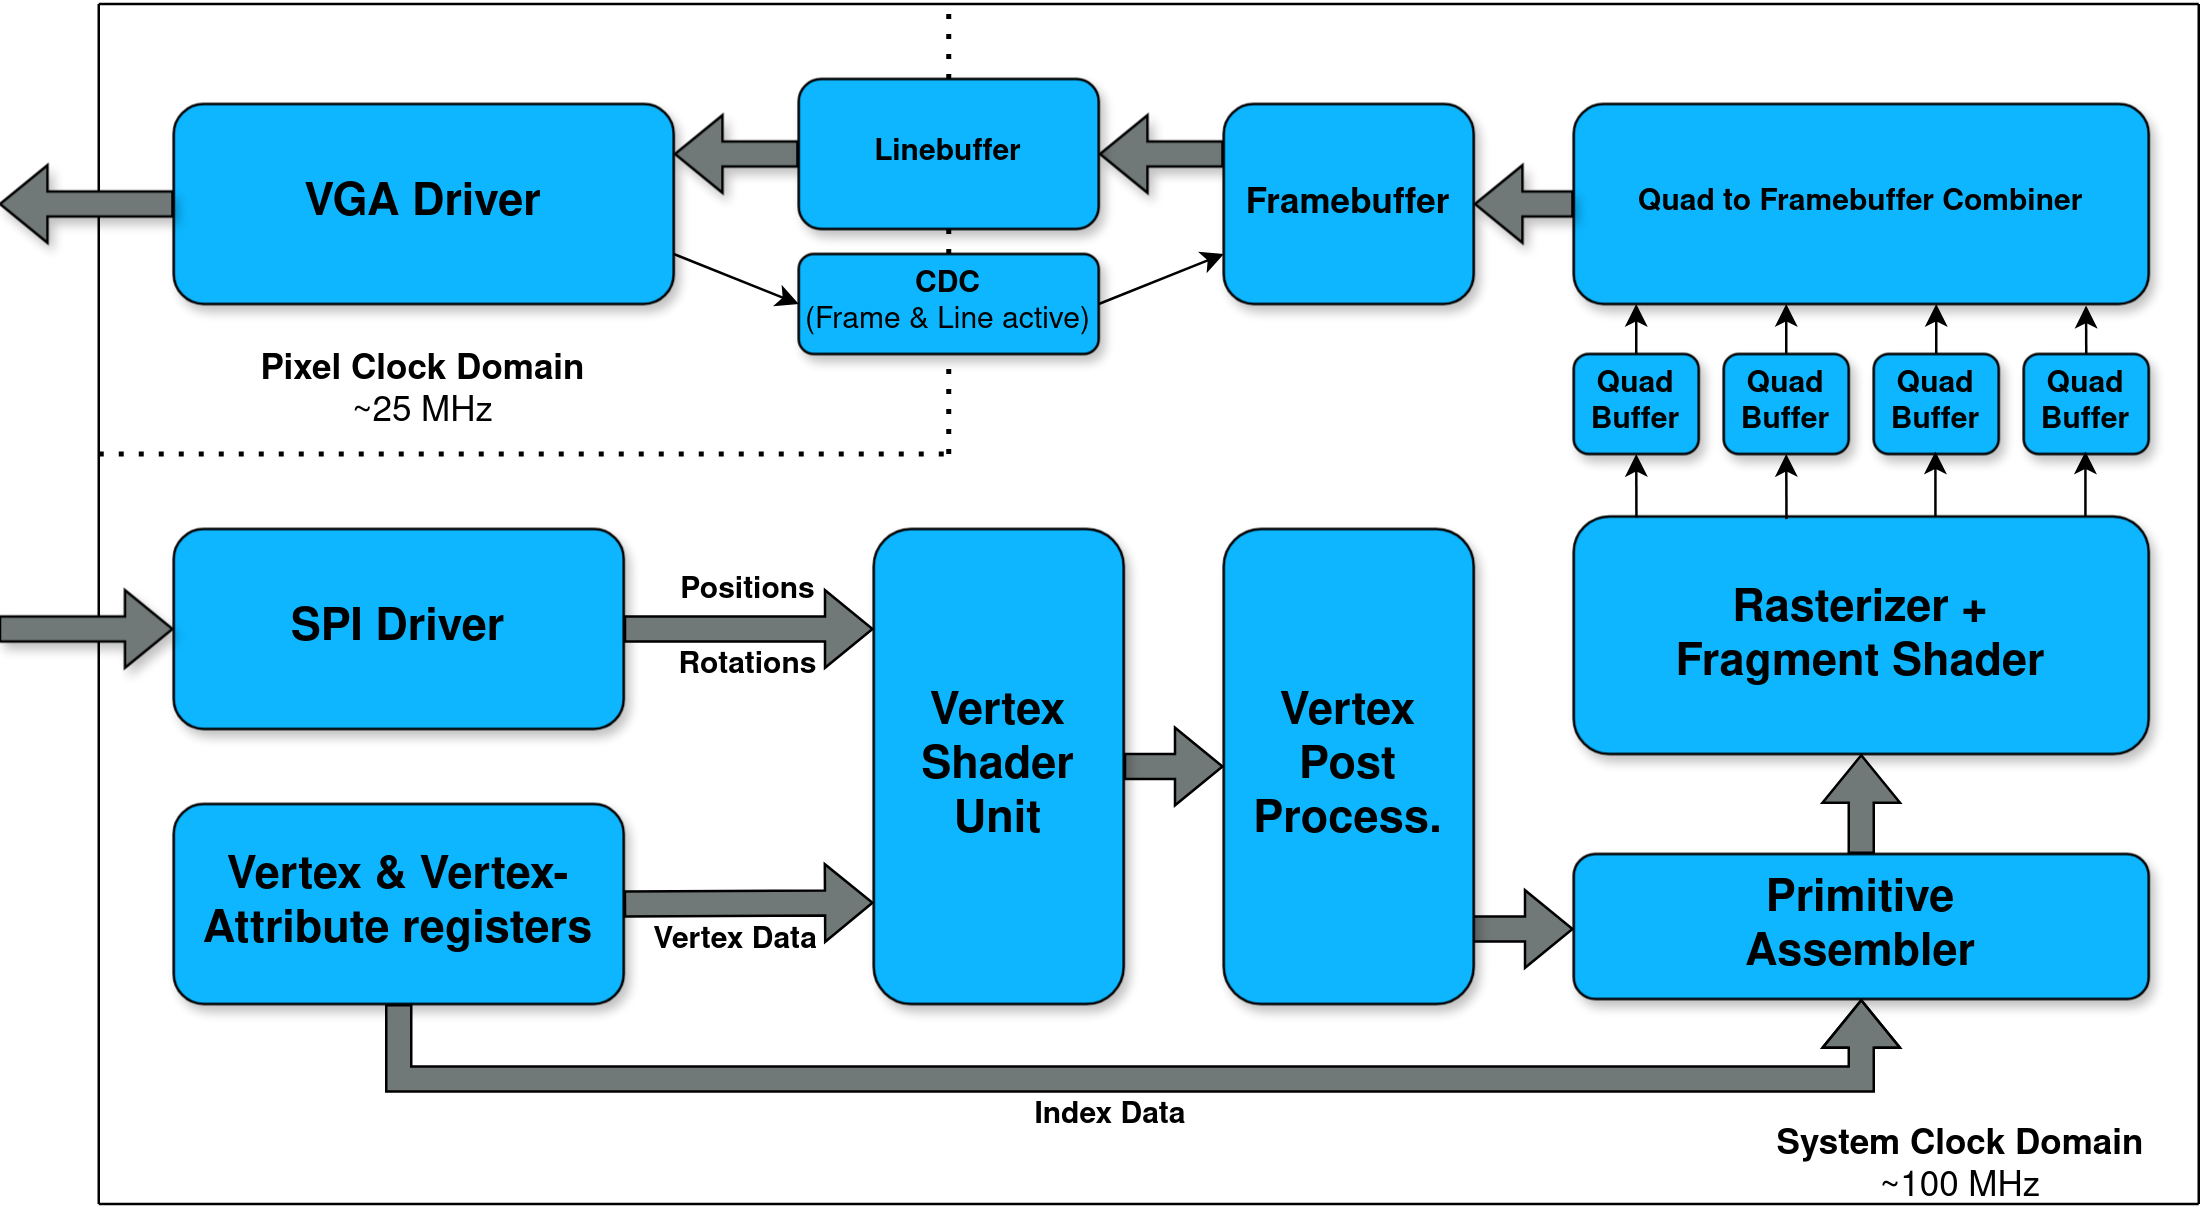
\includegraphics[width=0.95\textwidth]{Diagrams/fpga_system.png}
\end{figure}

The system has two main clock domains: the pixel clock domain for controlling the 
display at around $~\SI{25}{\mega\hertz}$, and the system clock domain for the rest 
of the system at around $\SI{100}{\mega\hertz}$.

The render pipeline is the main part of the system. It's what does the graphics 
processing, taking in mesh data and outputting pixels.
